\documentclass{article}
\usepackage[paperwidth=13.333in,paperheight=7.5in,margin=0in]{geometry}
\usepackage{tikz}
\usepackage{fontspec}
\usepackage{xcolor}
\usepackage{pagecolor}
\pagestyle{empty}
\setlength{\parindent}{0pt}
\setmainfont{Avenir Next}
\newfontfamily\displayfont{Iowan Old Style}
\usetikzlibrary{calc}

\definecolor{paper}{HTML}{EEF2F6}
\definecolor{ink}{HTML}{1A1F26}
\definecolor{muted}{HTML}{6F7882}
\definecolor{hair}{HTML}{D7E0E7}
\definecolor{accentred}{HTML}{B07A78}
\definecolor{accentblue}{HTML}{6D88A6}
\definecolor{accentgold}{HTML}{B6A07B}
\definecolor{leftcore}{HTML}{C88D89}
\definecolor{leftshoulders}{HTML}{DBB4AF}
\definecolor{leftouter}{HTML}{DCC3A3}
\definecolor{corridor}{HTML}{CDD5DC}
\definecolor{reservoir}{HTML}{8CB7B8}
\definecolor{funnel}{HTML}{98AED0}
\definecolor{cardfill}{HTML}{F8FAFC}

\begin{document}
\pagecolor{paper}

\noindent
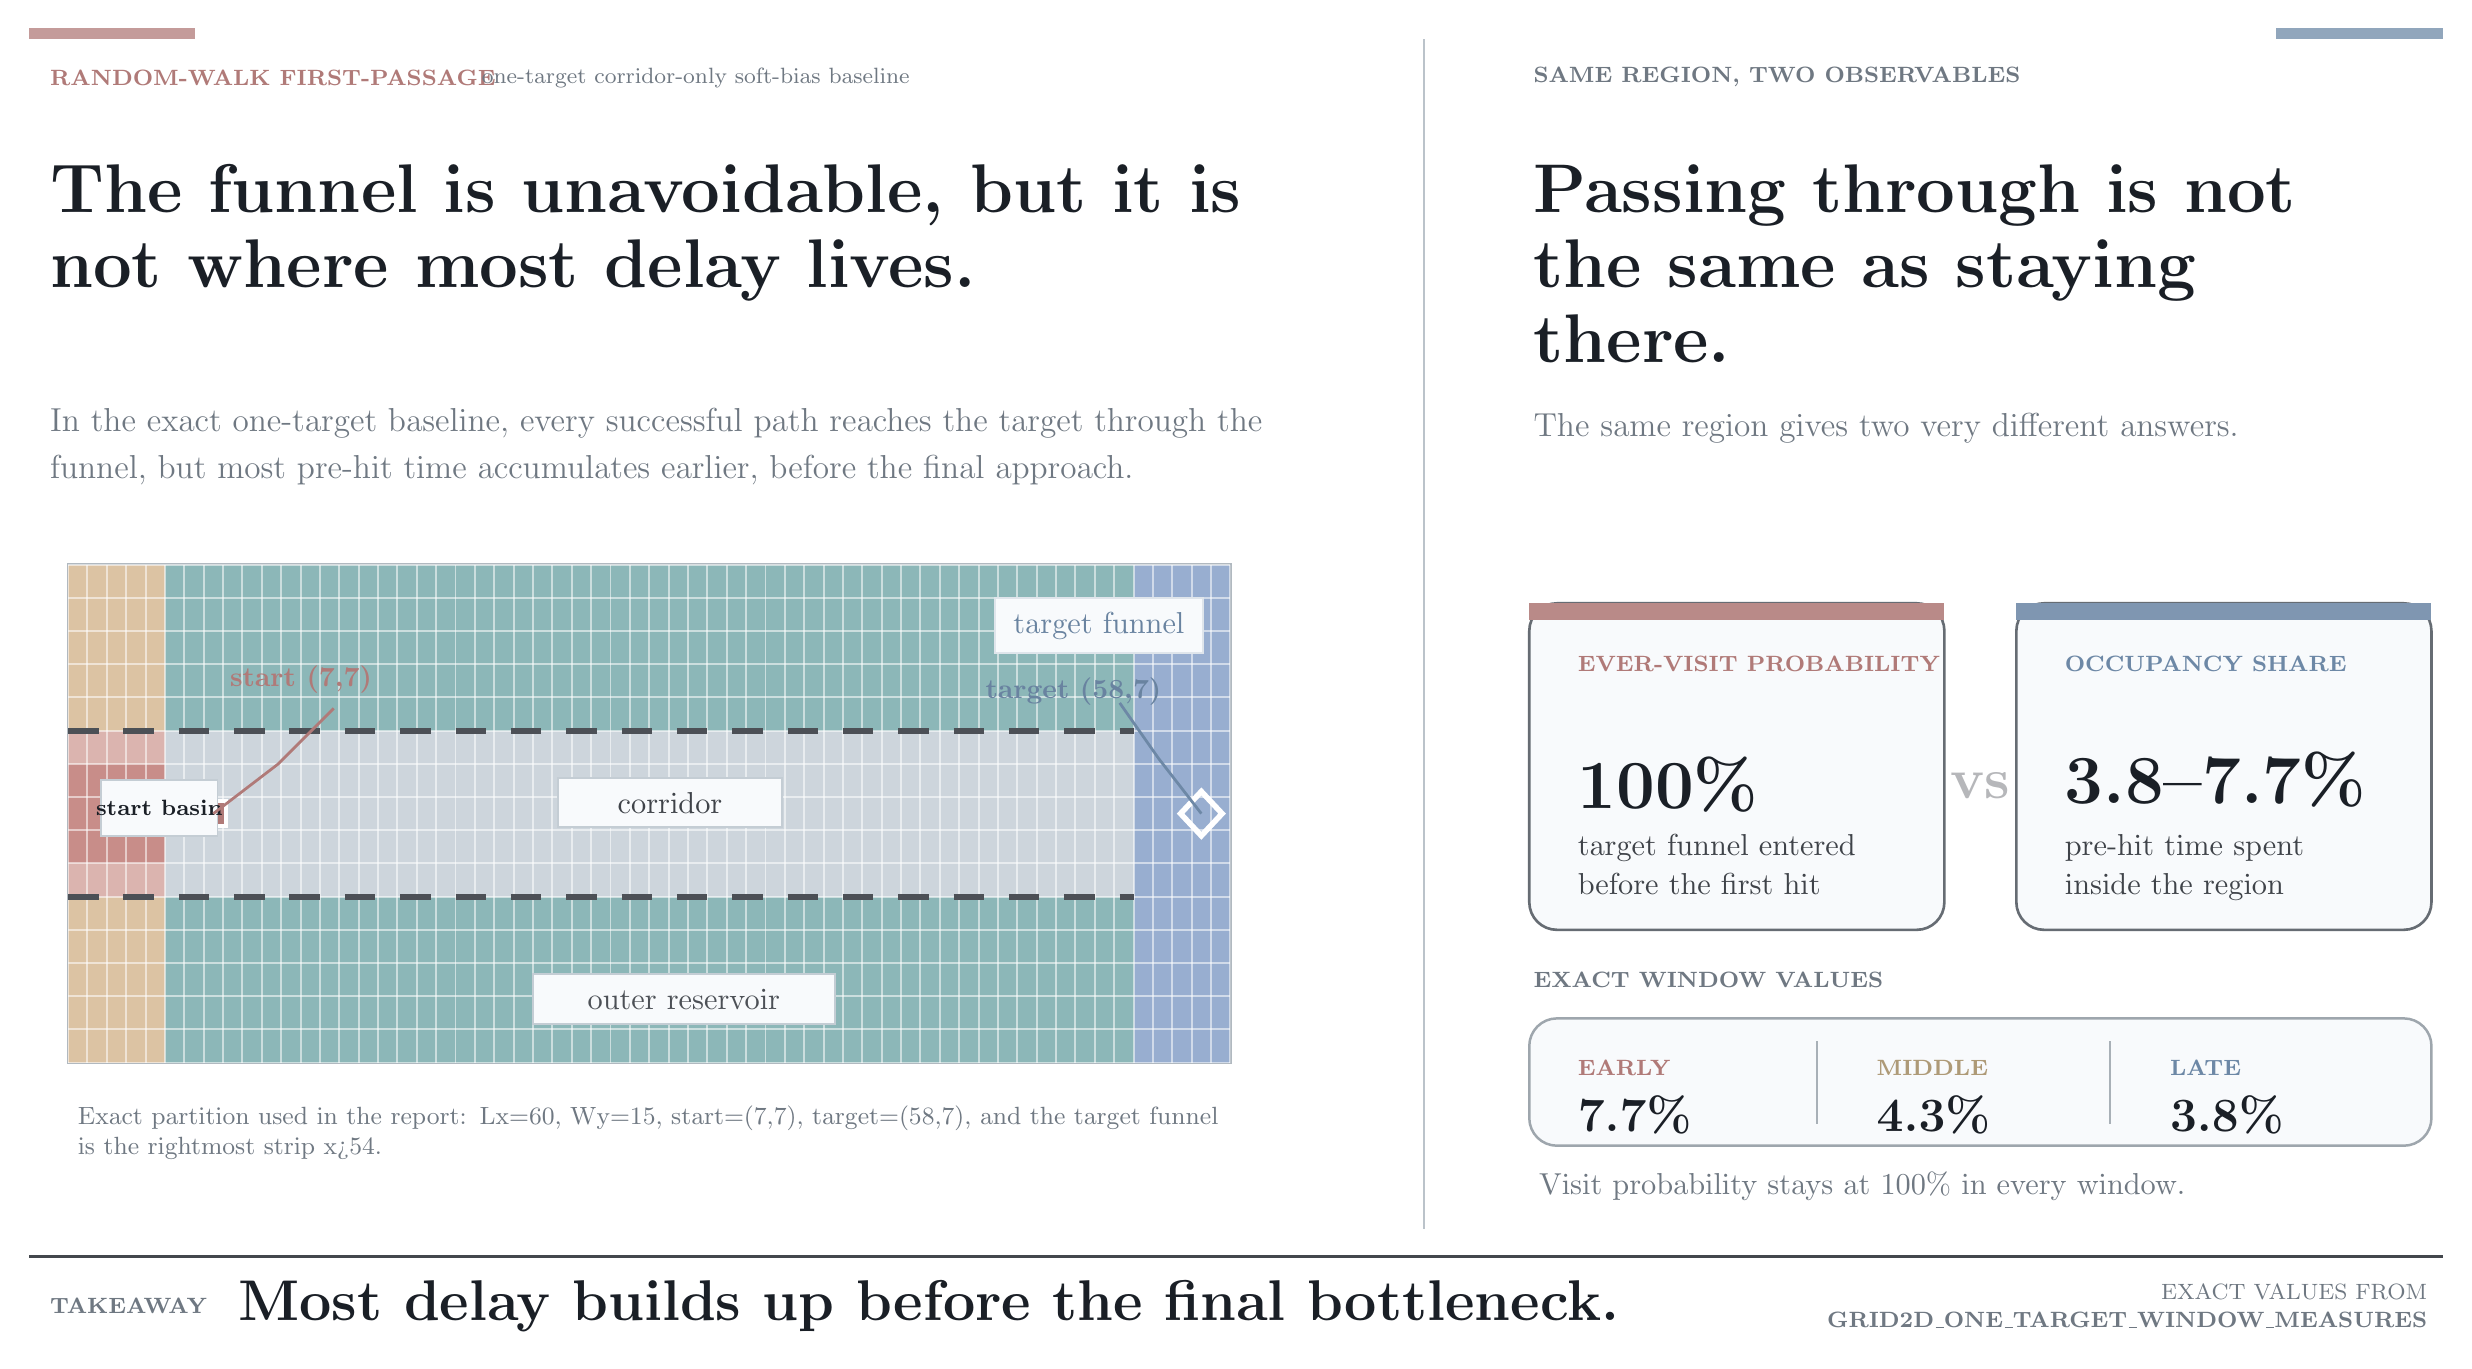
\begin{tikzpicture}[x=1pt,y=1pt]

% page accents
\fill[accentred!75] (44,500) rectangle (104,504);
\fill[accentblue!75] (856,500) rectangle (916,504);
\draw[hair!85!ink, line width=0.9pt] (548,70) -- (548,500);
\draw[ink!82, line width=1.2pt] (44,60) -- (916,60);

% left header
\node[anchor=west, text=accentred, font=\bfseries\fontsize{8}{8}\selectfont] at (48,486) {RANDOM-WALK FIRST-PASSAGE};
\node[anchor=west, text=muted, font=\fontsize{8}{8}\selectfont] at (204,486) {one-target corridor-only soft-bias baseline};
\node[anchor=north west, text=ink, font=\displayfont\bfseries\fontsize{24}{27}\selectfont, align=left, text width=468pt]
  at (48,458) {The funnel is unavoidable, but it is not where most delay lives.};
\node[anchor=north west, text=muted, font=\fontsize{13}{17}\selectfont, align=left, text width=458pt]
  at (48,370) {In the exact one-target baseline, every successful path reaches the target through the funnel, but most pre-hit time accumulates earlier, before the final approach.};

% left geometry frame
\begin{scope}[yshift=-8pt]
\draw[hair!80!ink, line width=1pt] (58,138) rectangle (478,318);

% exact partition map
\begin{scope}
  \clip (58,138) rectangle (478,318);

  % x cell = 7pt, y cell = 12pt, exact domain 60 x 15
  % outer regions
  \fill[leftouter] (58,138) rectangle (93,198);
  \fill[leftouter] (58,258) rectangle (93,318);
  \fill[leftshoulders] (58,198) rectangle (93,210);
  \fill[leftshoulders] (58,246) rectangle (93,258);
  \fill[leftcore] (58,210) rectangle (93,246);

  \fill[reservoir] (93,138) rectangle (443,198);
  \fill[reservoir] (93,258) rectangle (443,318);
  \fill[corridor] (93,198) rectangle (443,258);
  \fill[funnel] (443,138) rectangle (478,318);

  % grid
  \foreach \x in {58,65,...,478} {
    \draw[white, opacity=0.55, line width=0.7pt] (\x,138) -- (\x,318);
  }
  \foreach \y in {138,150,...,318} {
    \draw[white, opacity=0.55, line width=0.7pt] (58,\y) -- (478,\y);
  }

  % corridor boundaries
  \draw[ink!78, line width=2.2pt, dash pattern=on 11pt off 9pt] (58,198) -- (443,198);
  \draw[ink!78, line width=2.2pt, dash pattern=on 11pt off 9pt] (58,258) -- (443,258);

  % start = (7,7), centered on the exact lattice cell
  \fill[accentred] (106,223.5) rectangle (115,232.5);
  \draw[white, line width=1.3pt] (106,223.5) rectangle (115,232.5);

  % target = (58,7), centered on the exact lattice cell
  \draw[white, line width=2pt] (467.5,236) -- (475,228) -- (467.5,220) -- (460,228) -- cycle;

  % in-figure labels
  \fill[cardfill] (70,220) rectangle (112,240);
  \draw[hair!90!ink, line width=0.7pt] (70,220) rectangle (112,240);
  \node[font=\bfseries\fontsize{8}{8}\selectfont, text=ink] at (91,230) {start basin};

  \fill[cardfill] (235,223) rectangle (316,241);
  \draw[hair!90!ink, line width=0.7pt] (235,223) rectangle (316,241);
  \node[font=\fontsize{11}{11}\selectfont, text=ink!84] at (275.5,232) {corridor};

  \fill[cardfill] (226,152) rectangle (335,170);
  \draw[hair!90!ink, line width=0.7pt] (226,152) rectangle (335,170);
  \node[font=\fontsize{11}{11}\selectfont, text=ink!78] at (280.5,161) {outer reservoir};

  \fill[cardfill] (393,286) rectangle (468,306);
  \draw[accentblue!22, line width=0.7pt] (393,286) rectangle (468,306);
  \node[font=\fontsize{11}{11}\selectfont, text=accentblue!95!ink] at (430.5,296) {target funnel};
\end{scope}

% geometry callouts
\node[anchor=south west, text=accentred, font=\bfseries\fontsize{10}{10}\selectfont] at (113,268) {start (7,7)};
\draw[accentred, line width=1pt] (154,266) -- (134,246) -- (110.5,228);
\node[anchor=west, text=accentblue!95!ink, font=\bfseries\fontsize{10}{10}\selectfont] at (386,272) {target (58,7)};
\draw[accentblue, line width=1pt] (438,268) -- (452,248) -- (467.5,228);

\node[anchor=north west, text=muted, font=\fontsize{9}{11}\selectfont, align=left, text width=420pt]
  at (58,126) {Exact partition used in the report: Lx=60, Wy=15, start=(7,7), target=(58,7), and the target funnel is the rightmost strip x>54.};
\end{scope}

% right header
\node[anchor=west, text=muted, font=\bfseries\fontsize{8}{8}\selectfont] at (584,486) {SAME REGION, TWO OBSERVABLES};
\node[anchor=north west, text=ink, font=\displayfont\bfseries\fontsize{24}{27}\selectfont, align=left, text width=322pt]
  at (584,458) {Passing through is not\\the same as staying\\there.};
\node[anchor=north west, text=muted, font=\fontsize{11.5}{15}\selectfont, align=left, text width=310pt]
  at (584,368) {The same region gives two very different answers.};

% metric cards
\begin{scope}[yshift=-8pt]
\path[rounded corners=10pt, fill=cardfill, draw=hair!40!ink, line width=0.95pt] (586,186) rectangle (736,304);
\fill[accentred!88] (586,298) rectangle (736,304);
\node[anchor=west, text=accentred, font=\bfseries\fontsize{8}{8}\selectfont] at (600,282) {EVER-VISIT PROBABILITY};
\node[anchor=north west, text=ink, font=\bfseries\fontsize{31}{31}\selectfont] at (600,252) {100\%};
\node[anchor=north west, text=ink!84, font=\fontsize{10.5}{14}\selectfont, align=left, text width=120pt]
  at (600,224) {target funnel entered\\before the first hit};

\node[text=ink!32, font=\displayfont\bfseries\fontsize{20}{20}\selectfont] at (749,238) {vs};

\path[rounded corners=10pt, fill=cardfill, draw=hair!40!ink, line width=0.95pt] (762,186) rectangle (912,304);
\fill[accentblue!88] (762,298) rectangle (912,304);
\node[anchor=west, text=accentblue, font=\bfseries\fontsize{8}{8}\selectfont] at (776,282) {OCCUPANCY SHARE};
\node[anchor=north west, text=ink, font=\bfseries\fontsize{28}{28}\selectfont] at (776,254) {3.8--7.7\%};
\node[anchor=north west, text=ink!84, font=\fontsize{10.5}{14}\selectfont, align=left, text width=118pt]
  at (776,224) {pre-hit time spent\\inside the region};

% evidence section
\node[anchor=west, text=muted, font=\bfseries\fontsize{8}{8}\selectfont] at (584,168) {EXACT WINDOW VALUES};
\path[rounded corners=10pt, fill=cardfill, draw=hair!70!ink, line width=0.9pt] (586,108) rectangle (912,154);
\draw[hair!75!ink, line width=0.7pt] (690,116) -- (690,146);
\draw[hair!75!ink, line width=0.7pt] (796,116) -- (796,146);
\node[anchor=west, text=accentred, font=\bfseries\fontsize{8}{8}\selectfont] at (600,136) {EARLY};
\node[anchor=west, text=ink, font=\bfseries\fontsize{18}{18}\selectfont] at (600,119) {7.7\%};
\node[anchor=west, text=accentgold!95!ink, font=\bfseries\fontsize{8}{8}\selectfont] at (708,136) {MIDDLE};
\node[anchor=west, text=ink, font=\bfseries\fontsize{18}{18}\selectfont] at (708,119) {4.3\%};
\node[anchor=west, text=accentblue, font=\bfseries\fontsize{8}{8}\selectfont] at (814,136) {LATE};
\node[anchor=west, text=ink, font=\bfseries\fontsize{18}{18}\selectfont] at (814,119) {3.8\%};
\node[anchor=north west, text=muted, font=\fontsize{10.5}{12}\selectfont, align=left, text width=320pt]
  at (586,102) {Visit probability stays at 100\% in every window.};
\end{scope}

% bottom takeaway
\node[anchor=west, text=muted, font=\bfseries\fontsize{8}{8}\selectfont] at (48,42) {TAKEAWAY};
\node[anchor=west, text=ink, font=\displayfont\bfseries\fontsize{21}{23}\selectfont] at (116,42)
  {Most delay builds up before the final bottleneck.};
\node[anchor=east, text=muted, font=\fontsize{8}{10}\selectfont, align=right] at (914,42)
  {EXACT VALUES FROM\\\textbf{GRID2D\_ONE\_TARGET\_WINDOW\_MEASURES}};

\end{tikzpicture}

\end{document}
